\chapterquote{%
Although modeling is a central component of modern science, scientific models at best are approximations of the objects and systems that they represent—they are not exact replicas. Thus, scientists constantly are working to improve and refine models.}
{-- Kara Rogers, \textit{Scientific modeling} (2011)}

In the previous chapter, there was no analysis regarding retransmission performance (e.g. delay) and related parameters (e.g. retransmission rate).
%
This is done in this chapter\footnote{The present chapter was based on the article \cite{dester2021retrans}.}.

Our main motivation for this part is to analyze the impact of limiting the maximum number of allowed retransmissions $m\in\N$ for each packet.
%
When we increase $m$, the throughput $\mathscr{T}$ increases because fewer packets are discarded. On the other hand, the delay $D$ also increases because the packet stays longer in the system and contributes to increasing the aggregate interference (see Remark~\ref{remark:optimization}).
%
Indeed, we prove that selecting the smallest number of allowed retransmissions that satisfy some requirements is the optimal approach.

Another problem that arises because we have a loss system is that the delay metric ignores discarded packets.
%
Thus, an ``optimal'' solution may consider discarding some packets only because the associated delays are large. This would artificially decrease the mean packet delay.
%
That is why we will use the Age-of-Information (AoI) metric along with the delay.
%
This metric takes into account the time spent by dropped packets and is defined in the following section.

\begin{remark} \label{remark:optimization}
    Regarding the optimization of $m$, it is desirable to have a single metric that takes into account both $\mathscr{T}$ and $D$ in a meaningful way, however that is not an easy task.
    %
    Of course we could propose objective functions such as, for constant $w_0 > 0$,
    \begin{align*}
        \mathscr{T} - w_0\,D, \qquad \frac{\mathscr{T}}{D}, \qquad \mathscr{T} \euler^{-w_0\,D},
    \end{align*}
    or any bivariate function which monotonically increases with $\mathscr{T}$ and monotonically decreases with $D$. All these examples lead to a Pareto optimum\footnote{A Pareto optimum is a situation where no changes can be made that improves a metric without worsting off another.}, however they do not carry (\textit{a priori}) any physical interpretation.
    %
    To circumvent this choice dilemma, we optimize the delay $D$ and consider the throughput $\mathscr{T}$ as a constraint of the optimization.
    %
    Then, we do not have to worry about application specificities and we can tackle the problem in a more general form.
\end{remark}

% % % % % % % % % % % % % % % % % % % % % % % % 
% % % % % % % % % % % % % % % % % % % % % % % % 
\section{Age-of-Information metric}

For a given user, at time $t$, let $U(t)$ be the time the last received packet was generated. Then, the AoI metric is defined as $\Delta(t) \triangleq t-U(t)$ \cite{kaul2011minimizing, kaul2012real}.
%
Thus, it measures the delay to refresh the information on the receiver.

In this chapter, we use a related metric called \textit{Peak-Age-of-Information} (PAoI), which corresponds to the \textit{Age-of-Information} when a packet is successfully received.
%
The mean PAoI metric considers the time spent by dropped packets, which represents an important difference from the classical mean delay metric that may provide a misleading result when we have a high proportion of discarded packets.

In our model, we assume that the generation of packets is modelled as events that follow a Poisson process. Thus, discarding a packet too soon (small $m$) may have a high cost in the PAoI metric, because the node does not know when the next packet is coming.

For example, let us take the cases of no retransmissions ($m=0$), one allowed retransmission ($m=1$) and no limit for retransmissions ($m = \infty$). If there is a long wait between the arrival of packets with successful transmission, we may observe what is shown in Figure~\ref{fig:PAoI_examples}.
%
Without retransmissions, only the packets that arrive and are successfully transmitted contribute to decreasing the AoI. When we allow one retransmission, the packets that have success in the first retransmission also contribute, and so on.
%
Fig.~\ref{fig:PAoI_examples} illustrates why increasing $m$ decreases the mean PAoI in this case.
%
\begin{figure}[htb]
    \centering
    \if\printfig1
        \includegraphics[width=\textwidth]{Figures/Ch6_PAoI_Intro.pdf}
    \else
        \includegraphics[width=\textwidth,draft]{Figures/Ch6_PAoI_Intro.pdf}
    \fi
    \caption{Examples of measures of the PAoI metric for different retransmission strategies.}
    \label{fig:PAoI_examples}
\end{figure}

On the other hand, if retransmissions are performed several times and a new packet arrives before a successful retransmission happens, then the old packet is dropped and the retransmissions only served to generate interference, thus increasing the PAoI.
%
% However, we cannot forget that increasing $m$ increases aggregate interference, which may increase the PAoI in the end.

% % % % % % % % % % % % % % % % % % % % % % % % 
% % % % % % % % % % % % % % % % % % % % % % % % 
\section{Random Access Network with Limited Retransmissions}

In this section, we analyze the impact of a limited number of retransmissions in the network performance by tuning the number of allowed retransmissions $m\in\N$ and the rate $r\in\R_+$ at which the packet to be retransmitted will access the network.
%
Specifically, we consider a scenario where only the most recent event matters, and thus, a packet waiting to be retransmitted is dropped whenever a new packet arrives.

Our aim in this work is to select the optimal pair $r$ and $m$ for the metrics throughput, delay, and PAoI.
%
The main differences of our work from recent works {\cite{chen2020age1, chen2020age2, yates2017status}} are that we deal with a general transmission success probability function of the traffic, i.e., this can represent the collision model, the capture model, or any arbitrary model that does not depend directly on $r$ and $m$. Also, we consider limiting the maximum number of retransmissions to improve performance.
%
In this framework, we prove that selecting the smallest number of allowed retransmissions that satisfy some requirements is the optimal approach.

% In {\cite{chen2020age1, chen2020age2, yates2017status}}  {the transmission success probability is derived from the classical collision model;}
% %
% in \cite{chen2020age1}  {the authors propose a random access scheme to optimize the AoI for a set of arrival rates and a large number of nodes;}
% %
% in {\cite{chen2020age2}}  {the authors propose a random access scheme to optimize the AoI based on the instantaneous AoI of each node;}
% %
% in {\cite{yates2017status}}  {the authors show that random access perform worse than scheduled access with feedback by a factor of approximately $2\euler$ in the AoI.}

%-%-%-%-%-%-%-%-%-%-%-%-%-%-%-%-
\subsection{System Model}

Consider a single class stationary and ergodic network with a given number of nodes (possibly infinite), each node receives a packet whenever an event associated with that node occurs, and we suppose the events occur according to a Poisson process of parameter $a > 0$.
%
Thus, $a$ is also the arrival rate of packets per node. Once the packet arrives, the node transmits the packet\footnote{{This assumption can be easily modified to transmit the packet after an exponentially distributed time upon arrival without compromising the analytical tractability.}} to a receiver. If the packet is successfully transmitted, it is dropped\footnote{Successful reception acknowledgment is transmitted in an error-free channel.}.
%
Otherwise, the node transmits it again after an exponentially distributed time with a parameter $r > 0$, which is the retransmission rate.

In this scenario, we suppose that only the data related to the most recent event matter, i.e.,
% if a new packet arrives while the node is still trying to retransmit an older packet, then the latter is dropped and the new packet is transmitted.
if a new packet arrives, the old one waiting to be retransmitted is dropped. Another case where the packet is also dropped is when it reaches the number of allowed retransmissions $m \in \Z_+$.
%
To attain analytical tractability of the system model we further assume:
%
\begin{itemize}[itemsep=3pt,parsep=3pt,topsep=3pt,partopsep=3pt]
    \item stationary homogeneous traffic $\upsilon$ per unit of area, i.e., all receivers experience interference with the same distribution\footnote{
     {The main purpose of this assumption is to eliminate the intricate coupling and interactions between the transmitting nodes.}
    %
    This is valid in large-scale networks with high-mobility nodes, or with a small access probability \cite{haenggi2013diversity}, or with frequency hopping in several channels.};
    % \item the interference process is iid for each transmission\footnote{This is a valid assumption in high-mobility systems \cite{baccelli2010stochastic} or if there is frequency hopping in a sufficiently large number of channels \textcolor{red}{[Referência]}};
    \item transmission time is negligible compared with the waiting time to retransmit or for a new packet to arrive in the node;
    \item stationary success probability of a single transmission is a general function $p_s:\R_+\longrightarrow[0,1]$ of traffic $\upsilon$ that satisfies the conditions of Theorem~\ref{th:unique_opt}, which guarantees existence and uniqueness of the optimum throughput.
\end{itemize}

The first assumption along with having a single user class entail that the system throughput is a function of the traffic $\upsilon$ and it is given by $\mathscr{T}(\upsilon) = \upsilon\,p_s(\upsilon)$.

\begin{figure}[htb]
    \centering
    \if\printfig1
        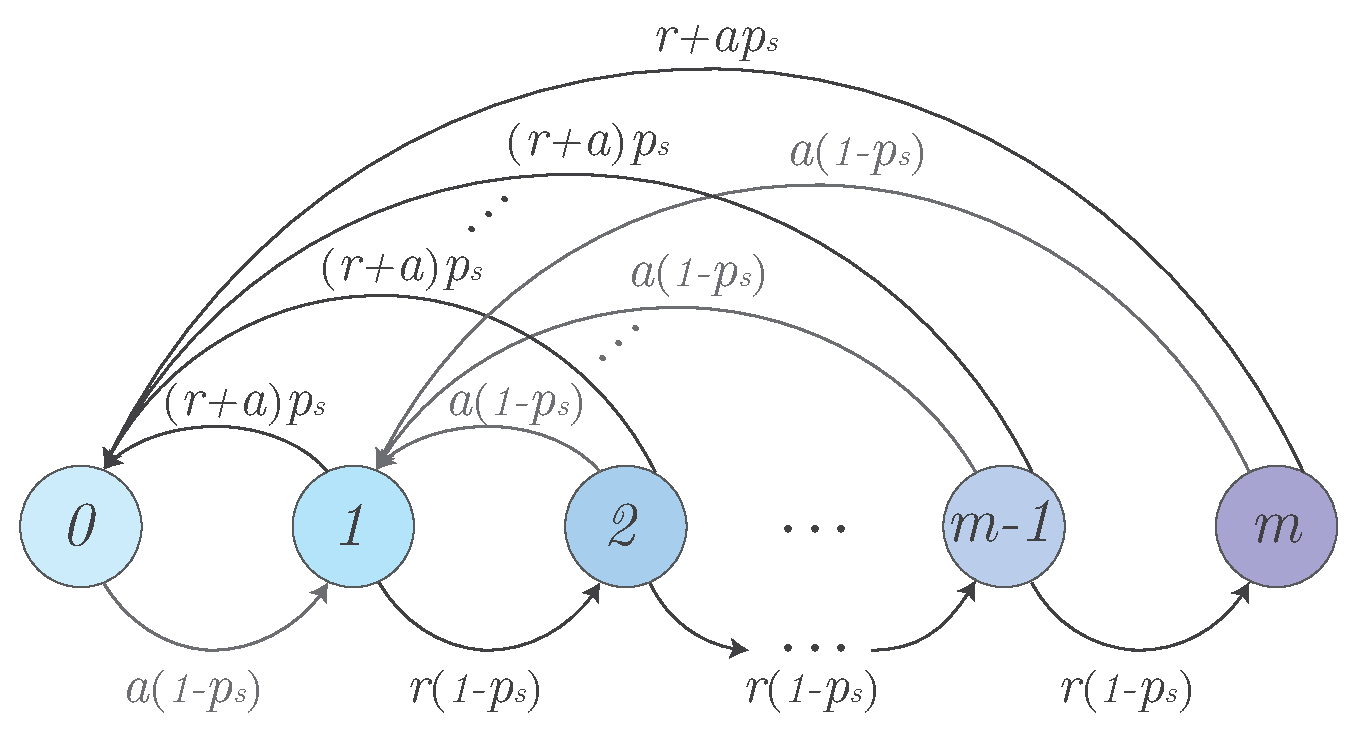
\includegraphics[width=0.6\textwidth]{Figures/Ch6_markch.pdf}
      %\includegraphics[width=\columnwidth]{images/markovDiagram.pdf}
    \else
        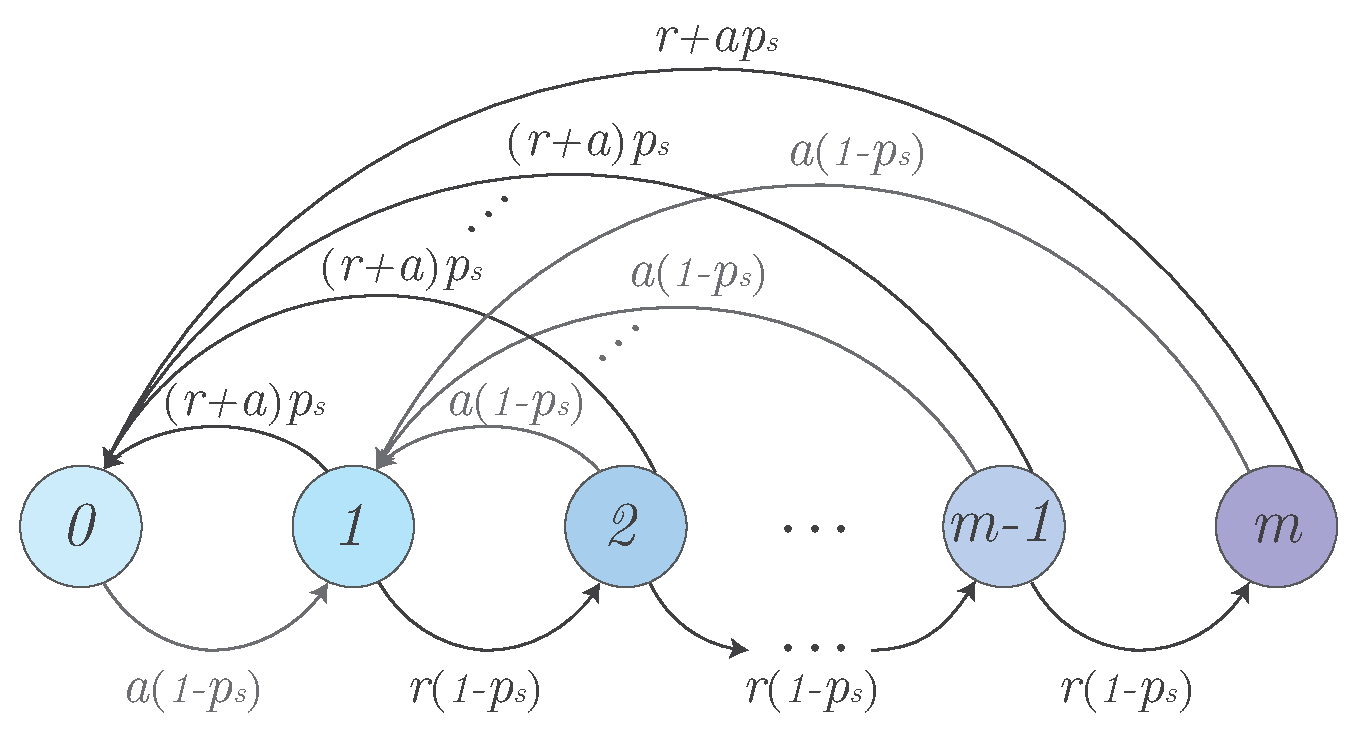
\includegraphics[draft,width=0.6\textwidth]{Figures/Ch6_markch.pdf}
    \fi
    \caption{Markov chain transition rates for a typical node.}
    \label{fig:markov_diagram}
\end{figure}

From now on, let us use $p_s$ to denote $p_s(\upsilon)$ to lighten the notation.

The state of a typical node can be represented as a continuous-time Markov chain with transition rates (Definition~\ref{def:transition-rate}):
\begin{align*}
    k \to k+1:&~ r\,(1-p_s), && 0 < k < m, \\
    k \to 1:&~ a\,(1-p_s),   && 0 \le k \le m, \\
    k \to 0:&~ (r + a)\,p_s, && 0 < k < m, \\
    m \to 0:&~ r + a\,p_s,
    % \text{otherwise}:&~ 0,
\end{align*}%
 {where the state $k\in\{1,2,\dots,m\}$ represents the number of transmissions that occurred with the buffered packet, and $k=0$ represents that the buffer is empty.}
%
These transition rates are illustrated in the diagram of Fig.~\ref{fig:markov_diagram}.
%, where $a$ is the arrival rate of new packets per node, $r$ is the rate of retransmission packets, $p_s$ is the packet success probability.
The nodes that are retransmitting have a transmission rate of $r+a$ because they can transmit either by retransmission or when a new packet arrives.
%
The nodes that are not retransmitting ($k=0$) have a transmission rate of $a$.

More specifically,
%
the transition $k\to k+1$ represents an unsuccessful retransmission (with probability $1-p_s$), which occurs at rate $r$;
%
the transition $k\to 1$ represents an unsuccessful transmission (with probability $1-p_s$) of an arriving packet, which occurs at rate $a$;
%
the transition $k\to 0$ corresponds to a successful transmission (with probability $p_s$), which can be from a retransmitted packet (rate $r$) or arriving packet (rate $a$);
%
finally, the transition $m\to 0$ corresponds to a successful or unsuccessful transmission, because in this state ($m$ retransmissions) the packet is dropped even with failure.

In view of the general network model of Chapter~\ref{cap:P2_00} we provide a possible example of a network that fits the above assumptions.
%
\begin{example} 
    Consider a stationary and ergodic high-mobility bipolar Poisson network with one user class and density of transmitters $\lambda_{\S}>0$ on the plane $\S=\R^2$, transmission time $\tau_i = \tau$ and transmission power $P_i \equiv 1$ for every user $i\in\N$, and link distance $r_0 > 0$.
    
    For each transmitter $i\in\N$, suppose packets arrive according to a Poisson point process $A_i$ of density $a>0$ on time $\T = \R$. Each transmitter can access the channel according to a Poisson point process $U_{i}$ of density $r>0$ or if a packet arrived. Thus, transmissions can happen according to the point process $T_i = A_i + U_i$. However, they only happen if there is a packet in the buffer, thus transmissions will happen according to the thinned point process $T^*_{i} = q_i\,T_i$, where the function $q_i = \ind\{Q_i(t) > 0\}$, and the queue dynamics of $Q_i$ is defined such that it follows the continuous-time Markov process presented in Figure~\ref{fig:markov_diagram}.
    
    Furthermore, assuming Rayleigh fading, path loss function $\ell(x) = x^{-\alpha}$, $\alpha>2$, and the \textit{capture model} with threshold $\theta>0$ for the transmission success probability, then according to Theorem~\ref{prop:PPP_ps} we have that
    \begin{align*}
        p_s = \exp\!\left( -\upsilon \pi r_0^2 \theta^\delta \frac{\delta\pi}{\tau\sin(\delta\pi)} \right),
    \end{align*}
    where $\delta\triangleq 2/\alpha$.
    
    Thus, $p_s$ essentially depends on the traffic $\upsilon$ and other constants. Therefore, the system model presented in this section applies to this network.
\end{example}

Let us define $\{\pi_k\}_{k\in\Z_+}$ as the stationary probabilities of the typical node being in the $k$th retransmission.
%
Then, in the stationary state, the network traffic is given by%
\begin{align} \label{eq:traffic_ret}
    \upsilon &= \frac{\upsilon_0}{a} \left( a \pi_0 + (r+a) (1-\pi_0) \right) = \upsilon_0 \left( 1 + \frac{r}{a} (1 - \pi_0) \right),
\end{align}
where $\upsilon_0$ is the traffic without retransmission, i.e., if $r=0$, then $\upsilon=\upsilon_0$.
%
It is important to remember that $p_s$ depends on the traffic of the system, and thus, we have a challenging problem because $\upsilon$ also depends on $p_s$ owing to the dependence on the stationary probabilities. % See Proposition~\ref{prop:pi} in the following section.
The following section circumvents this problem and presents the analytical results.

%-%-%-%-%-%-%-%-%-%-%-%-%-%-%-%-
\subsection{Analysis}

Let us assume that the packet arrival rate $a$ and the traffic without retransmissions $\upsilon_0$ are fixed and known.
%
Our objective here is to optimize the retransmission rate $r$ and the number of allowed retransmissions $m$ in view of some performance metrics.
%
We begin by solving the Markov chain of Fig.~\ref{fig:markov_diagram} for its stationary probabilities.
%
The following proposition gives us the stationary probabilities (Definition~\ref{def:markov-defs}) of the Markov chain.

\begin{proposition} \label{prop:pi}
    The stationary probability $\pi_k$ of finding the typical node in the $k$th retransmission state is given by
    \begin{align*}
        % \pi_0 &= 1 - \frac{a}{r}\,\frac{1-p_s}{p_s +a/r}\left(1-\left(\frac{1-p_s}{1+a/r}\right)^m\right),\\
        \pi_0 &= 1 - \frac{a}{r} \frac{\xi\,(1-\xi^m)}{1-\xi},\\
        \pi_k &= \frac{a}{r}\,\xi^k, \qquad 1\le k\le m,
    \end{align*}
    where $\xi \triangleq \dfrac{r(1-p_s)}{r+a}$ is the retransmission probability.
\end{proposition}

\begin{proof}
    From the Markov chain transition probabilities, we have that, for $2\le k\le m$,
    $
        (r+a)\pi_k = r (1-p_s) \pi_{k-1}.
    $
    Thus, $\pi_k = \left(\frac{r(1-p_s)}{r+a}\right)^{k-1}\pi_1$.
    Using this relation along with
    \begin{align*}
        a(1-p_s)\pi_0 &= (r+a)p_s\sum_{k=1}^m\pi_k + r(1-p_s) \pi_m,\\
        r(1-p_s)\pi_1 &= (r p_s+a)\sum_{k=2}^m\pi_k + r(1-p_s) \pi_m,
    \end{align*}
    and $\sum_{k=0}^m \pi_k = 1$, we find the desired solution.
\end{proof}

Using Proposition~\ref{prop:pi}, we can rewrite \eqref{eq:traffic_ret} in the simpler form
\begin{align} \label{eq:traffic_ret2}
    \upsilon = \frac{1-\xi^{m+1}}{1-\xi} \upsilon_0.
\end{align}

Let $\upsilon^*\in\R_+$ be the traffic for which we have the maximum throughput $\mathscr{T}^* = \upsilon^* p_s^*$, where $p_s^* = p_s(\upsilon^*)$. Theorem~\ref{th:unique_opt} guarantees the existence and uniqueness of $\upsilon^*$.
%
The optimum traffic $\upsilon^*$ can be found by solving the equation $\psi(\upsilon^*) = 1$, where $\psi$ is defined in Theorem~\ref{th:unique_opt}.
%
We can achieve $\upsilon^*$ by adjusting the retransmission rate to an appropriate $r^*$ for each $m\in\Z_+$.

When $m=1$,\vspace{-5mm}
\begin{align}
    r^* = \frac{a(\upsilon^*-\upsilon_0)}{(2-p_s^*)\upsilon_0 - \upsilon^*}, \quad\text{if}~ \frac{\upsilon^*}{2-p_s^*} < \upsilon_0 \le \upsilon^*.
\end{align}

When $m = \infty$, i.e., unlimited number of retransmissions,
\begin{align} \label{eq:opt_retr_rate}
    r^* = \frac{a\,(\upsilon^*-\upsilon_0)}{\upsilon_0 - p_s^* \upsilon^*}, \quad\text{if}~ p_s^* \upsilon^* < \upsilon_0 \le \upsilon^*.
\end{align}

As expected, the inequality on $\upsilon_0$ when $m=1$ is more strict than for $m = \infty$, since we can achieve greater traffic with the latter.
%
For general $m\in\N$, we have the following result.

\begin{lemma} \label{lem:max_lam}
    For all $r\in\R_+$, $m\in\N$,
    % \begin{align*}
    %     \frac{\upsilon}{\upsilon_0}
    %         = \frac{1-(1-p_s)^{m+1}}{p_s}.
    % \end{align*}
    \begin{align*}
        1 \le \frac{\upsilon}{\upsilon_0} \le \frac{1-(1-p_s)^{m+1}}{p_s}.
    \end{align*}
\end{lemma}
%
\begin{proof}
    First, let us prove that for a fixed $p_s$, we have 
    $
        {\frac{\partial \upsilon}{\partial r} \ge 0}.
    $
    \begin{align*}
        \frac{\partial \upsilon}{\partial r} = \upsilon_0\, \frac{a/r}{a+r}\, \frac{\beta^{m+1} - m(\beta-1)-\beta}{\beta^m (\beta-1)^2},
    \end{align*}
    where $\beta\triangleq \xi^{-1} \ge 1$. Notice that the expression
    \begin{align*}
        \beta^{m+1} - m(\beta-1)-\beta &= (1+(\beta-1))^{m+1} - (m+1)(\beta-1) - 1 \\
            &= \left(\sum_{k=0}^{m+1} \binom{m+1}{k} (\beta-1)^k\right)- (m+1)(\beta-1) - 1\\
            &= \sum_{k=2}^{m+1} \binom{m+1}{k} (\beta-1)^k \\ &\ge 0.
    \end{align*}
    Therefore,
    $
        {\frac{\partial \upsilon}{\partial r}\ge 0}.
    $
    Then, $\displaystyle \upsilon_0 \le \upsilon \le \lim_{r\to\infty} \upsilon$, from which we conclude the proof through the calculation of the limit.
\end{proof}

A consequence of Lemma~\ref{lem:max_lam} is that to achieve the optimum traffic $\upsilon^*$ we must have
\begin{align} \label{eq:opt_cond}
    \frac{p_s^*\upsilon^*}{1-(1-p_s^*)^{m+1}} < \upsilon_0 \le \upsilon^*.
\end{align}

There might exist several values for $m$ that satisfy \eqref{eq:opt_cond}.
%
Let us focus on the optimal choice in view of some performance metrics.

% % % % % % % % % % % % % % % % % % % % % 
\subsubsection{Stationary Mean Delay}

% The throughput $\mathscr{T} = \upsilon\,p_s$ can also be calculated as the product of the traffic without retransmissions $\upsilon_0$ and the probability that a packet is not dropped, i.e., $\mathscr{T} = \upsilon_0 \, \P(D < \infty)$, where 
Let $D$ be the \textit{improper} random variable that represents the delay of a typical packet. If it is dropped, then ${D=\infty}$.
%
From the Markov chain and the fact that the sum of exponential iid random variables follows an Erlang distribution, we can show that the cdf of $D$ is
\begin{align*}
    F_D(t) = p_s + \int_0^t f_D(t)\,\d t, \qquad 0\le t < \infty,
\end{align*}
where
\begin{align}
    f_D(t) = \sum_{k=1}^m p_s\,\xi^k \frac{ (r+a)^k t^{k-1}}{(k-1)!} \,\euler^{-(r+a) t}, \qquad t\in\R_+.
        % &= p_s\delta_0(t) + p_s \xi\,(r+a) \frac{\Gamma\left(m, \xi\,(r+a) t\right)}{\Gamma(m)}\,\euler^{-(1-\xi) (r+a) t}, \nonumber
\end{align}

\begin{note}
    Note that the rate associated with the Erlang distribution to calculate the function $f_D$ is the sum of the rate of retransmission $r$ with the rate of arrival $a$ instead of simply $r$.
    %
    This might be counter-intuitive because we are conditioning on the event of retransmitting the packet to calculate the delay.
    %
    This is associated with the following interesting problem.
    
    Let $X, Y$ be independent random variables that follow exponential distributions of parameters $\alpha$ and $\beta$, respectively.
    %
    Let $0 < \alpha < \beta$, $t\in\R_+$. We invite the reader to compare, without calculations, the probabilities $\P(\min(X,Y)\le t)$ and $\P(\min(X,Y)\le t \mid X \le Y)$.

    For independent $X\sim\mathscr{E}(\alpha)$ and $Y\sim\mathscr{E}(\beta)$, standard calculations show the possibly counter-intuitive result
    $\P(\min(X,Y)\le t) = 1 - \euler^{-(\alpha+\beta)t} = \P(\min(X,Y)\le t \mid X \le Y).$
    
    That is, $\min(X,Y) \sim \mathscr{E}(\alpha+\beta)$ and $\min(X,Y) \mid X \le Y \sim \mathscr{E}(\alpha+\beta)$.
    %
    We say counter-intuitive because we could, for example, expect that $\min(X,Y) \mid X \le Y \sim \mathscr{E}(\alpha)$.

    % \begin{align*}
    %     \P(\min(X,Y)\le t)
    %         &= 1 - \P(\min(X,Y) > t) \\
    %         &= 1 - \P(X > t, Y > t) \\
    %         &= 1 - \P(X > t)\,\P(Y > t) \\
    %         &= 1 - \euler^{-(a+b)t}.
    % \end{align*}
    
    % \begin{align*}
    %     \P(\min(X,Y)\le t \mid X \le Y)
    %         &= \frac{\P(\min(X,Y)\le t, X \le Y)}{\P(X \le Y)} \\
    %         &= \frac{\P(X \le t, X \le Y)}{\P(X \le Y)}\\
    %         &= \dfrac{\displaystyle \int_0^t f_X(x) \left( \int_x^\infty f_Y(y) \d y \right) \d x}{\displaystyle \int_0^\infty f_X(x) \left( \int_x^\infty f_Y(y) \d y \right) \d x} \\
    %         &= 1 - \euler^{-(a+b)t}.
    % \end{align*}
    
    In our original problem, this means that conditioning on the event of having retransmission does not reduce the rate to $r$, i.e., it continues to be the sum of the retransmission and the arrival rates $r+a$.
\end{note}

\begin{note}
    Note that $f_D$ is not the pdf of $D$. The pdf does not exist (with respect to the Lebesgue measure) as discussed in Note~\ref{note:dirac_function}, because the events $\{D=0\}$ and $\{D=\infty\}$ have positive probability measures.
\end{note}

The event of packet success is equivalent to $D<\infty$, thus the packet success probability
%
\begin{align} \label{eq:pps}
    p_p = \P(D<\infty) = p_s\frac{1-\xi^{m+1}}{1-\xi}.
\end{align}
%
As expected, this satisfies $\upsilon_0 p_p = \upsilon p_s = \mathscr{T}$. %, because it is another form of calculating the throughput.

Then, the mean delay of a successfully transmitted packet, which we shall define as
\begin{align} \label{eq:delay}
    \overline{D} \triangleq \E[D\mid D<\infty] &= \frac{\int_0^\infty t\, f_D(t)\, \d t}{\P(D<\infty)} 
        % &\quad = \frac{1-p_s}{p_s r+a}
        % \left( \frac{1 - \left(1 + m\frac{p_s+a/r}{1+a/r}\right) \left(\frac{1-p_s}{1+a/r}\right)^m}{1 -  \left(\frac{1-p_s}{1+a/r}\right)^{m+1} } \right).
        = \frac{1}{r+a}\left(\frac{1}{1-\xi} - \frac{1+m\xi^{m+1}}{1-\xi^{m+1}}\right).
\end{align}

% % % % % % % % % % % % % % % % % % % % % 
\subsubsection{Stationary Mean PAoI}
%
\begin{figure}[htb]
    \centering
    \if\printfig1
        \includegraphics[width=0.7\columnwidth]{Figures/Ch6_PacketRetransmission_PAoI.pdf}
    \else
        \includegraphics[draft,width=0.85\columnwidth]{Figures/Ch6_PacketRetransmission_PAoI.pdf}
    \fi
    \caption{Time evolution of the \textit{Age-of-Information} metric. The \textit{Peak-Age-of-Information} $A^{(n)}$ is the measure of the \textit{Age-of-Information} when a packet is successfully transmitted. In this example, the first dropped packet is due to reaching the maximum number of retransmissions ($m=2$) and the second dropped packet is due to the arrival of a new packet.
    %
    Except for the discontinuities, note that the AoI is always increasing with slope $1$, because it measures the time since the generation of the last correctly received packet.
    %
    Also note that $Y^{(n)}$ comprises the time between the arrival of packets that are successfully transmitted, i.e., the first and the fourth packet in this case.
    }
    \label{fig:PAoI_diagram}
\end{figure}

The random variable PAoI $A^{(n)}$ measures the time between the $n$th successfully received packet transmission and the previous successfully received packet generation. It is defined as
\begin{align}\label{eq:A}
    A^{(n)} = Y^{(n)}+T^{(n)},
\end{align}
where $Y^{(n)}$ is the interarrival time between packets of a typical node that are not dropped, and $T^{(n)}$ is the time a packet that is not dropped spends in the system, i.e., $\E[T^{(n)}] = \overline{D}$.

Fig.~\ref{fig:PAoI_diagram} shows a realization of the stochastic process with $m=2$ and two dropped packets.
%
% whenever it applies for all $n$. The random variable $Y$ is composed of the time spent with a successfully transmitted packet plus a packet arrival, as illustrated in Fig.~\ref{fig:PAoI_diagram}, which shows a realization of the stochastic process with $m=2$ and two dropped packets. Then,
The random variable $Y^{(n)}$ is composed by
\begin{align}\label{eq:Y}
    Y^{(n)} = T^{(n-1)} + B^{(n)} + \sum_{i=1}^{K^{(n)}} L^{(n)}_i,%
\end{align}%
where $B\sim\mathscr{E}(a)$ %follows an exponential distribution of the parameter $a$ and 
represents the packet arrival time since the last successful transmission (memoryless property),
%
$K\sim\mathscr{G}(p_p)$ %follows a geometric distribution of parameter $p_p$ and
represents the number of dropped packets until the arrival of a packet that is not dropped,
%
and $L_i$ is the time spent by the $i$th dropped packet since its arrival until a new packet arrives, its distribution is decribed in the proof of Proposition~\ref{prop:meanPAoI}. % which is independent from $T$ and $\{L_i\}_i$.
%
% A realization of the stochastic process, where we have $m=2$ and two dropped packets, is shown in Fig.~\ref{fig:PAoI_diagram}.

A closed-form expression for the mean PAoI metric is given by the following proposition.

\begin{proposition}\label{prop:meanPAoI}
    The stationary mean PAoI is given by
    \begin{align} \label{eq:PAoI}
        \E[A] &= \frac{1}{a}\!+\!\frac{1}{a+r} \frac{1-\xi^m}{1-\xi^{m+1}}
            \left( \frac{1-p_s}{p_s} + \frac{\xi}{1-\xi} - \frac{m\xi^{m+1}}{1-\xi^m} \right)\nonumber\\
            &\quad + \frac{1}{a}(1-p_s)\,\xi^m\left(\frac{1-\xi}{p_s\,(1-\xi^{m+1})}-1\right).
    \end{align}
    %
    Also,\qquad\qquad
    $\displaystyle
        \lim_{m\to\infty}\E[A] = \frac{1}{a} + \frac{1}{a+r}\left(\frac{1-p_s}{p_s} + \frac{\xi}{1-\xi}\right).
    $
\end{proposition}
\begin{proof}
    Using the Markov chain we can show that the moment generating function of $L$ and its expectation is given by
    
    \begin{align}
        M_L(t) &= \E[\euler^{-t L}] \nonumber\\
            &= \frac{1}{\P(D\!=\!\infty)} \bigg( \sum_{k=1}^m (1-p_s-\xi)\xi^{k-1} \left( 1 - \frac{t}{r+a} \right)^{-k} \nonumber\\
            &\qquad + (1-p_s) \xi^m \left( 1 - \frac{t}{r+a} \right)^{-m}\left( 1 - \frac{t}{a} \right)^{-1} \bigg),\nonumber\\
        \E[L] &= \left. \frac{\d}{\d t} M_L(t) \right|_{t=0} \label{eq:EL} \nonumber\\ 
            %\frac{1 - p_s - \xi - \xi^m (p_s (m (\xi -1) \xi -1)-\xi +1)}        {(r+a)(1 -\xi)\left(1-\xi-p_s(1-\xi^{m+1})\right)}\nonumber\\
            &= \frac{1}{r+a}\left( \frac{1}{1-\xi} - \frac{\xi^m(1-p_s(1+m\xi))}{1-\xi-p_s(1-\xi^{m+1})} \right) + \frac{1}{a}(1-p_s)\xi^m.
    \end{align}
    %
    % Also,
    % \begin{align*}
    %     \lim_{m\to\infty} \E[L] = \frac{1}{(r+a)(1-\xi)}.
    % \end{align*}
    % It is possible to find a closed form for the distribution of $Y$ (for example, through generating functions), however the final expression is so cumbersome that it will not help in any way.
    
    Using \eqref{eq:A}, \eqref{eq:Y} and taking the expectation gives us
    \begin{align*}
        \E[A] 
            = \E[Y] + \E[T]
            % &= \E[B] + 2\,\E[T] + \sum_{k=0}^\infty p_p \P(D=\infty)^k k\,\E[L] \\
            = a^{-1} + 2\,\overline{D} + \E[K] \E[L].
    \end{align*}
    % This metric takes into account not only the mean delay of a successful packet, but the total delay in updating the information caused by the unsuccessful packets as well.
    % %
    % Indeed, this metric is objectively more demanding than the mean delay, since the expected number of dropped packets between successful transmissions $\E[K]$ decreases with $m$.
    
    Then, using \eqref{eq:pps}, \eqref{eq:delay}, and \eqref{eq:EL} concludes the proof.
\end{proof}

% % % % % % % % % % % % % % % % % % % % % 
\subsubsection{Retransmission Optimization}
Finally, we can state the main result of the present chapter.%
\begin{proposition} \label{prop:best_m}
    Let $\upsilon\in\R_+$. If $\upsilon_0 \in (\upsilon p_s(\upsilon), \upsilon)$,
    then there exist infinite pairs of retransmission rates $r\in\R_+$ and number of allowed retransmissions $m\in\Z_+$ that achieve the network traffic $\upsilon$. Furthermore, the pair with the smallest $m$ has the minimal mean delay $\overline{D}$ and mean PAoI $\E[A]$.
\end{proposition}
%
\begin{proof}
    If $p_s \upsilon < \upsilon_0 < \upsilon$, then there exist an infinite number of pairs $m,r$ that we can choose to reach the desired traffic $\upsilon$, because for each integer $m$ that satisfies Lemma~\ref{lem:max_lam} there exists a unique $r\in\R_+$ that achieves the traffic $\upsilon$, by the fact that $\partial\upsilon/\partial r > 0$ from the proof of Lemma~\ref{lem:max_lam}.
    
    After some tedious manipulations using the definition of $\xi$ along with \eqref{eq:traffic_ret2}, we can rewrite \eqref{eq:delay} and \eqref{eq:PAoI} as
    \begin{align*}
        \overline D &= \frac{1-p_s-\xi}{ a\,(1-p_s)(1-\xi)} \left( \xi - (\Upsilon+\xi-1) \frac{\ln\!\left(\frac{\Upsilon}{\Upsilon+\xi-1}\right)}{\ln(1/\xi)} \right),\\
        \E[A] &= \frac{1}{a}\Bigg[ 1 + (\Upsilon-p_s)\frac{1-p_s}{p_s} \frac{\Upsilon+\xi-1}{\xi\Upsilon} + \frac{1-p_s-\xi}{\xi\,(1-p_s)} (1-\Upsilon) \times\\
            &\qquad\qquad \left(\frac{1-p_s}{p_s} + \frac{\xi}{1-\xi}
              - \frac{\xi\,(\Upsilon+\xi-1) \ln\!\left(\frac{\xi\Upsilon}{\Upsilon+\xi-1}\right)}{(1-\xi)(1-\Upsilon)\ln(1/\xi)} \right) \Bigg],
    \end{align*}
    where $\Upsilon \triangleq \upsilon_0/\upsilon$ is fixed. Further, from Lemma~\ref{lem:max_lam} we can state that $0 \le 1-\Upsilon \le \xi \le 1-p_s \le 1$.
    %
    Then, we can show that $\frac{\partial \overline D}{\partial \xi} \le 0$ and $\frac{\partial \E[A]}{\partial \xi} \le 0$ as $\xi\in(1-\Upsilon,1-p_s)$.
    %
    We know that $m$ decreases with $\xi$ for a fixed $\Upsilon$ (see \eqref{eq:traffic_ret2}), then to achieve the smallest mean delay and mean PAoI, we must use the smallest $m$. This concludes the proof.
\end{proof}

% Minimizing the PAoI is harder than minimizing the delay, in the sense that the PAoI takes into account the time spent by unsuccessful packets until a successful transmission occurs, i.e., it is a more demanding version of the mean delay metric, which only takes into account the time spent by successful packets and might not be ideal as a performance measure of a network with a high packet dropping rate.

Given a requirement (constraint) among the metrics throughput $\mathscr{T}$, network traffic $\upsilon$, and packet success probability ${p_p}$, we should use the smallest number of allowed retransmissions $m$ such that we can adjust the retransmission rate $r$ to achieve the requirement and satisfy Lemma~\ref{lem:max_lam}.
%
Then, according to Proposition~\ref{prop:best_m}, we minimize both the metrics mean delay $\overline{D}$ and mean PAoI $\E[A]$.

\begin{figure}[htb]
\centering
    \begin{subfigure}[t]{.45\textwidth}
      \centering
        \if\printfig1
            \includegraphics[width=\columnwidth]{Figures/Ch6_opt_m.pdf}
            % 
\begin{tikzpicture}[scale = 0.85]

\begin{axis}
[
  title={},
%   width = 212.4pt,
%   width=12cm, height=9cm,
  legend style={at={(0.95,0.95)}, anchor=north east},
  xlabel={$p_s$},
  ylabel={$\dfrac{\upsilon_0}{\upsilon}$}, ylabel style={rotate=-90},
%  yticklabel=\pgfmathprintnumber{\tick}\\ \%,
  xmin = 0,
  xmax = 1,
  ymin = 0,
  ymax = 1,
%   y tick label style={
%         /pgf/number format/.cd,
%         fixed,
%         fixed zerofill,
%         precision=3,
%         /tikz/.cd
%   },
%   grid = both,
  scale only axis,
]
	\legend{}
    
    \foreach \m in {1,...,20}
        \addplot[thick, domain=0.001:1, samples=100]{x/(1-(1-x)^(\m+1))};

    % \foreach \m in {7,9,...,29}
    %     \addplot[thick, domain=0.001:1]{x/(1-(1-x)^(\m+1))};

    % \foreach \m in {30,40,...,100}
    %     \addplot[thick, domain=0.001:1]{x/(1-(1-x)^(\m+1))};
        
    \addplot[name path=A, thick, domain=0.0001:1, samples=100]{x/(1-(1-x)^(21+1))};
    \addplot[name path=B, thick, domain=0:1]{x};
    \addplot[black] fill between[of=A and B];
%     \addplot[blue, dashed] table
%     [
% 		x expr = \thisrow{lam_a}/0.2,
%     	y expr = \thisrow{p_r}
%     ] {./Data/p_th_old.dat};
%     \addplot[green!70!black, dashed] table
%     [
% 		x expr = \thisrow{lam_a}/0.2,
%     	y expr = \thisrow{p_a}
%     ] {./Data/p_th_old.dat};
    
    \fill[color=red!10] (axis cs: 0,0) -- (axis cs: 1,1) -- (axis cs: 1,0);
    
    \draw (axis cs: 0.10,0.70) node[anchor= west] {\large $m=1$};
    \draw (axis cs: 0.10,0.45) node[anchor= west, rotate=15] {\large $m=2$};
    \draw (axis cs: 0.10,0.33) node[anchor= west, rotate=20] {\large $m=3$};
    \draw (axis cs: 0.15,0.229) node[anchor= west, rotate=90] {$\cdots$};
    
    \draw (axis cs: 0.50,0.25) node[anchor= west]
        {\large
        \begin{tabular}{c}
            The traffic $\upsilon$ \\
            is not\\
            achievable
        \end{tabular}
        };
    
    % \node[text width=15mm,anchor=north east] at (1.04,1.07)
    %     {\tiny
    %     \begin{align*}
    %         a   &=0.40\\
    %             &=0.30\\
    %             &=0.20\\
    %             &=0.10\\
    %             &=0.05
    %     \end{align*}
    %     };
\end{axis}

\end{tikzpicture}

        \else
            \includegraphics[draft, width=\columnwidth]{Figures/Ch6_opt_m.pdf}
        \fi
        \caption{Optimal choice of $m$ for a given traffic $\upsilon$.}
        \label{fig:opt_m}
    \end{subfigure}%
    \begin{subfigure}{.05\textwidth}
        \hspace{.05\textwidth}
    \end{subfigure}%
    \begin{subfigure}[t]{.45\textwidth}
      \centering
        \if\printfig1
            \includegraphics[width=\columnwidth]{Figures/Ch6_opt_m_v2.pdf}
            % \input{Plots/Ch6_opt_m_v2}
        \else
            \includegraphics[draft,width=\columnwidth]{Figures/Ch6_opt_m_v2.pdf}
        \fi
        \caption{Optimal choice of $m$ for a given throughput $\mathscr{T}$ or packet success probability $p_p$.}
        \label{fig:opt_m_v2}
    \end{subfigure}
    \caption{}
\end{figure}

Fig.~\ref{fig:opt_m} shows the regions of the $\upsilon_0/\upsilon \times p_s$ plane for which we can choose the best value of the maximum number of retransmissions $m$ when the requirement is a given traffic $\upsilon$.
%
Fig.~\ref{fig:opt_m_v2} is similar to Fig.~\ref{fig:opt_m}, but now for the $\mathscr{T}/\upsilon_0 \times p_s$ plane.

If $p_s^* \upsilon^* < \upsilon_0 \le \upsilon^*$ we can choose as requirement the maximum throughput $\mathscr{T}^*$ or, equivalently, the optimum traffic $\upsilon^*$ and, then, use the figures to find the best value for $m$.
%
The following section provides a numerical example.

%-%-%-%-%-%-%-%-%-%-%-%-%-%-%-%-
\subsection{Numerical Example}

Let us study a simple scenario where the packet success probability function is $p_s(\upsilon) = \euler^{-\alpha\upsilon}$, for some parameter $\alpha>0$. Then, it is easy to show that the maximum throughput is achieved at $\upsilon^* = 1/\alpha$. Then, $p_s^* = 1/\euler$ and $\mathscr{T}^* = (\alpha\euler)^{-1}$.
%
Let us consider that the traffic without retransmission is given by $\upsilon_0 = a \lambda$, where $\lambda > 0$ is a quantity related to the number of users (e.g., the mean number of users per unit of area).

Then, we can plot the mean PAoI (Fig.~\ref{fig:PAoI_a}) as a function of the rate of packets per user $a$, which is a fixed and known quantity in the original problem. This is done for each number of allowed retransmissions $m\in\Z_+$ that satisfies Lemma~\ref{lem:max_lam} with $\upsilon=\upsilon^*$, so that we can adjust the retransmission rate $r^*$ and achieve the maximum throughput $\mathscr{T}^*$.

\begin{figure}[htb]
    \centering
    % \input{Plots/D_a.tex}%
    % \includegraphics[]{Figures/D_a.eps}%
    % \caption{mean delay $\overline D$ as a function of $a$ and for maximum throughput.\vspace{5mm}}
    % \label{fig:D_a}
    %
    \if\printfig1
        % 
\begin{tikzpicture}[scale=0.85]

\begin{axis}
[
  title={},
%   width=12cm, height=9cm,
  width = 0.65\columnwidth,
  legend style={at={(0.95,0.95)}, anchor=north east},
  xlabel={$a$},
  ylabel={mean PAoI [units of time]}, ylabel style={rotate=0},
%  yticklabel=\pgfmathprintnumber{\tick}\\ \%,
  xmin = 0,
  xmax = 1,
  ymin = 0,
  ymax = 8,
%   y tick label style={
%         /pgf/number format/.cd,
%         fixed,
%         fixed zerofill,
%         precision=3,
%         /tikz/.cd
%   },
  grid = both,
  scale only axis,
]
	\legend{}
    
    \addplot[name path=A, dashed] table
	[
		x expr = \thisrow{a},
    	y expr = \thisrow{PAoIinf}
    ] {./Data/PAoI_a_2_part1.dat};
    
    \addplot[name path=B, thick] table
	[
		x expr = \thisrow{a},
    	y expr = \thisrow{PAoIsup}
    ] {./Data/PAoI_a_2_part1.dat};
    
    \addplot[green!10] fill between[of=A and B];
    
    
    \addplot[name path=A, thick] table
	[
		x expr = \thisrow{a},
    	y expr = \thisrow{PAoIinf}
    ] {./Data/PAoI_a_2_part2.dat};

    \addplot[name path=B, thick] table
	[
		x expr = \thisrow{a},
    	y expr = \thisrow{PAoIsup}
    ] {./Data/PAoI_a_2_part2.dat};
    
    \addplot[green!10] fill between[of=A and B];

%%%%%%%%%%%%%%%%%%%%%%%%%%%%%%%%%%%%%%%%%%%%%%%%%%%%%%%%%%

    \addplot[name path=A, dashed] table
	[
		x expr = \thisrow{a},
    	y expr = \thisrow{PAoIinf}
    ] {./Data/PAoI_a_1_part1.dat};
    
    \addplot[name path=B, thick] table
	[
		x expr = \thisrow{a},
    	y expr = \thisrow{PAoIsup}
    ] {./Data/PAoI_a_1_part1.dat};
    
    \addplot[blue!10] fill between[of=A and B];
    
    \addplot[name path=A, thick] table
	[
		x expr = \thisrow{a},
    	y expr = \thisrow{PAoIinf}
    ] {./Data/PAoI_a_1_part2.dat};

    \addplot[name path=B, thick] table
	[
		x expr = \thisrow{a},
    	y expr = \thisrow{PAoIsup}
    ] {./Data/PAoI_a_1_part2.dat};
    
    \addplot[blue!10] fill between[of=A and B];

    
    \foreach \m in {2,...,10}
        \addplot[] table
    	[
    		x expr = \thisrow{a},
        	y expr = \thisrow{m\m}
        ] {./Data/PAoI_1_m234.dat};
    \foreach \m in {2,...,10}
        \addplot[] table
    	[
    		x expr = \thisrow{a},
        	y expr = \thisrow{m\m}
        ] {./Data/PAoI_2_m234.dat};


    \draw[-\arrowhead] (axis cs: 0.70, 1.80) -- (axis cs: 0.55, 3.80);
    \draw (axis cs: 0.55, 3.70) node[anchor= west] {\footnotesize ~$m = 1,2,\dots,\infty$};
    
    \draw[-\arrowhead] (axis cs: 0.40, 4.30) -- (axis cs: 0.25, 7.00);
    \draw (axis cs: 0.25, 7.00) node[anchor= west] {\footnotesize ~$m = 1,2,\dots,\infty$};

    % \draw (axis cs: 0.45,2.00) node[rotate=-20] {\footnotesize$\alpha\lambda_s=1$};
    % \draw (axis cs: 0.20,4.30) node[rotate=-40] {\footnotesize$\alpha\lambda_s=2$};
    \draw (axis cs: 0.43,1.95) node[rotate=-20] {\footnotesize$\alpha\lambda=1$};
    \draw (axis cs: 0.22,4.10) node[rotate=-30] {\footnotesize$\alpha\lambda=2$};

\end{axis}

\end{tikzpicture}
%
        \includegraphics[]{Figures/Ch6_PAoI_a.pdf}
    \else
        \includegraphics[draft, width=\textwidth]{Figures/placeholder.png}
    \fi
    % \includegraphics[width=0.73\columnwidth]{Figures/PAoI_a_v2.eps}%
    \caption{Mean PAoI $\E[A]$ as a function of $a$ for the maximum $\mathscr{T}$.}
    \label{fig:PAoI_a}
\end{figure}

The blue and green areas correspond to the optimum operating point (adjusting $r\in\R_+$) for each $m\in\N^*\cup\{\infty\}$ and $a\in[1/(\alpha\lambda\euler),1/(\alpha\lambda)]$. The green area is from a system that has twice as many users as the blue area system.
%
As expected, Proposition~\ref{prop:best_m} is observed in Fig.~\ref{fig:PAoI_a}, i.e., the smaller the number of allowed retransmissions $m$, the smaller the mean PAoI.
%
Further, we can see that as we increase $m$, the PAoI performance deteriorates. On the other hand, the region for which we can achieve the maximum throughput increases. For example, to achieve the maximum throughput when $a=1/2$ and $\alpha\lambda=1$, we need $m>1$. More precisely, $m=2$ from Fig.~\ref{fig:opt_m}, since $\upsilon_0/\upsilon^* = 1/2$ and $p_s = 1/\euler\approx 0.368$.
% This is in accordance with Lemma~\ref{lem:max_lam}, and Proposition~\ref{prop:best_m}.

% In Fig.~\ref{fig:D_a}, the mean delay of successful packets is close to $0$ whenever $\upsilon^*$ is close to $\upsilon_0$ ($= a \lambda$) or $p_s^* \upsilon_0$, for which $r^*$ tends to $0$ and $\infty$, respectively. In both cases, the delay tends to $0$, but this is a consequence of our assumption that the transmission time is negligible and in these edge cases it would no longer be valid.
%, because the percentage of dropped packets tends to $1$.
% This is one of the reasons we also used the mean PAoI metric, which elegantly takes into account the data transmission delay caused by dropped packets, so it can no longer be zero.

\begin{remark}
    In our problem, the arrival rate $a$ and initial traffic $\upsilon_0$ are fixed. If such quantities were free, the best approach would be to adjust them and use $m=1$ with a sufficiently small $r$.
\end{remark}

% % % % % % % % % % % % % % 
\section{Summary} \label{sec:summ_P2_02}

In this chapter, we studied a single class random access wireless network with homogeneous traffic, general transmission success probability function, and a retransmission scheme where packets are dropped when new packets arrive at the node or the number of allowed retransmissions is reached.

For a given throughput (or traffic or packet success probability) requirement, we showed that the best approach is to use the minimum number of allowed retransmissions such that, along with an appropriate retransmission rate, the desired requirement is achievable.
%
This approach is optimal for two different metrics: mean delay and mean \textit{Peak-Age-of-Information} (PAoI).
%
This suggests that choosing the smallest number of allowed retransmissions that achieves the network requirements could be an interesting design heuristic.